
\article{Инструмент}{Кустарь-одиночка с мотором}{

\href{https://www.youtube.com/playlist?list=PL6mXlWgvuzAu4jMVzOOKXXDVF3r1yAaz4}{Отличная
серия видео по изготовлению токарника}\bigskip

Возникает вопрос, где взять самый дешевый, легко доставаемый и универсальный
электропривод, и нужно ли вообще пользоватся электричеством.

Вопрос по использованию электричества оставляем самым упоротым \scr ам 80-го
левела. Будем исходить из того, что хоть какое-то (под нагрузку мощностью от
100$\div$200\,Вт) сетевое электричество доступно сейчас всем, кроме туристов,
огородников и прочих полевиков, не укомплектованных бензогенератором.

\emph{Соответственно в комплекте базового инструмента предполагаем наличие
минимум электродрели и паяльника.}

\subarticle{Электроинструмент}

\subsubarticle{Дрелъ}

\begin{multicols}{2}
\noindent\href{http://leroymerlin.ru/catalogue/instrumenty/elektroinstrument/dreli\_udarnye/13805983/}{
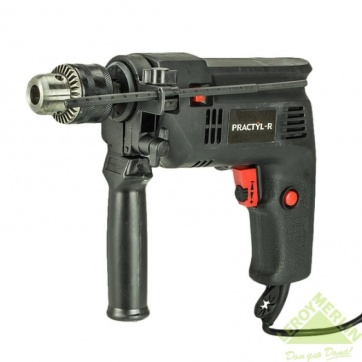
\includegraphics[width=\columnwidth]{00/fig/PraktylR.jpg}}
\textbf{Дрель ударная сетевая Praktyl-R PID13D01 400\,Вт (!)395\,р.}

\columnbreak

\noindent\href{http://leroymerlin.ru/catalogue/instrumenty/elektroinstrument/dreli\_bezudarnye/11857763/}{
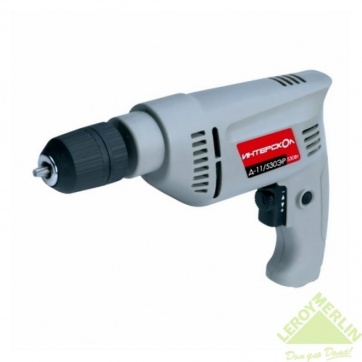
\includegraphics[width=\columnwidth]{00/fig/D_11_530ER.jpg}}
\textbf{Дрель безударная сетевая Интерскол Д-11/530ЭР (с БЗП) 1120\,р.}
\end{multicols}

Дрель\ --- одноразовая китайчатина от 400\,р. Цена крайне низкая, поэтому в
целях тестирования взял один экземпляр на натурные испытания, результаты по
живучести будут в следующих номерах. Подаются уже брендированные на Леруа
Мерлен, наклейка <<PID13D01 Ударная дрель 400\,Вт, 13\,мм>>. Скорость
регулируется глубиной нажатия курка, крутилка на курке ограничивает глубину
механически, фиксатор держит скорость близко к минимальной, запаха горелой
пластмассы через несколько минут работы на холостом ходу нет.

По надежности рекомедуется Интерскол
1100+\,р. Надежность Интерскола\ --- не <<китай>>, классика ДУ-580ЭР
работает в хвост и гриву в университете ежедневно с $\sim$2005 г., используется
криворукими студентами, лежит в подвале в пыли от точила, и никаких вопросов
даже со щетками.

Если не планируете много сверлить бетон, \textbf{берите дрель без ударного
механизма}: отсутствуют лишние продольные перемещения, что может быть важно при
использовании в качестве шпинделя сверлильного станка, и механизации других
технологических поделок.

\emph{Шуруповерт\ --- буржуйство, у него нет 43\,мм шейки для фиксации, поэтому
как средство электропривода он практически бесполезен, и нужен собственно для
заворачивания большого количества саморезов. Хотя наличие ограничителя
крутящего момента и малые габариты удобны при сверлении и сборке поделок.}

\subsubarticle{Лобзик}

\begin{multicols}{2}
\noindent\href{http://leroymerlin.ru/catalogue/instrumenty/elektroinstrument/lobziki/13805991/}{
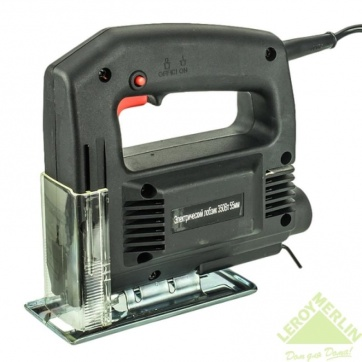
\includegraphics[width=\columnwidth]{00/fig/LobzPraktyl.jpg}}
\textbf{Лобзик Praktyl 350 Вт 356\,р.}

\columnbreak

\noindent\href{http://leroymerlin.ru/catalogue/instrumenty/elektroinstrument/lobziki/12114283/}{
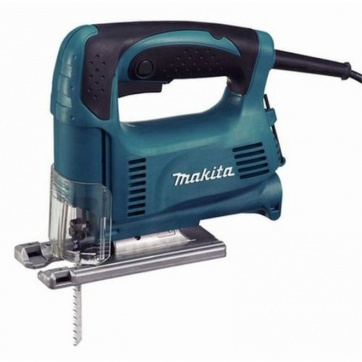
\includegraphics[width=\columnwidth]{00/fig/LobzMakita4329.jpg}}
\textbf{Лобзик Makite 4329 2260\,р.}
\end{multicols}

Лобзик опционален, и куда полезнее шуруповерта, китай-хлам 350+\,р, чуть
поприличнее 2000+\,р. \textbf{Не берите с маятником дешевле 5--7\,тыс.р}.

\subarticle{Паяльник}

\begin{multicols}{2}
\noindent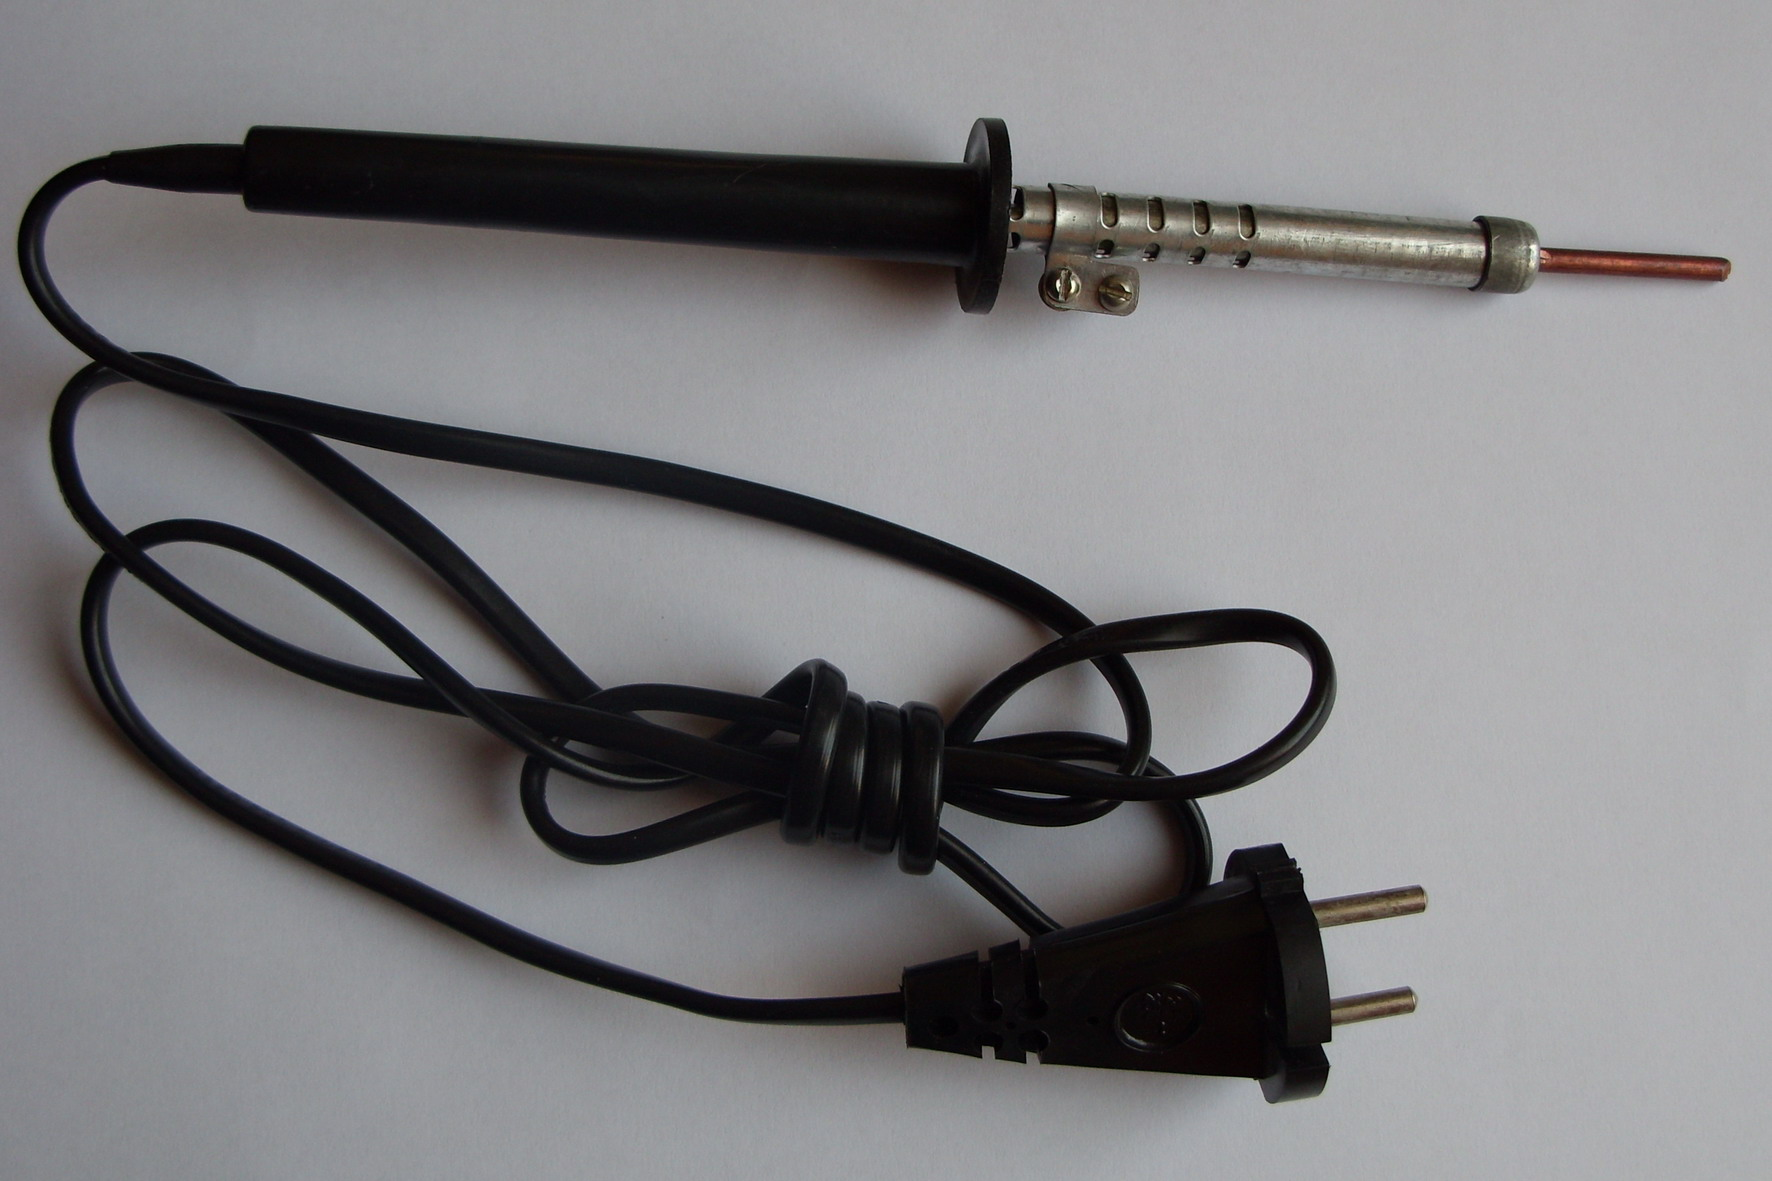
\includegraphics[width=\columnwidth]{00/fig/EPSN25.jpg}
\textbf{Паяльник ЭПСН-25/220}

\columnbreak

\noindent\href{http://voltmaster-samara.ru/catalog/product/00067650/}{
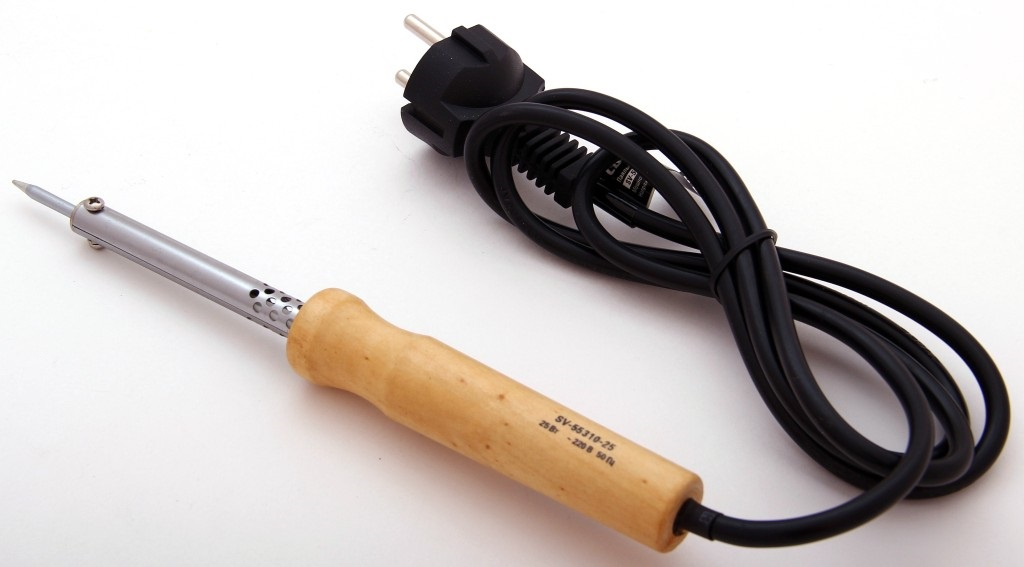
\includegraphics[width=\columnwidth]{00/fig/SV-55310-25.jpg}}
\textbf{Паяльник 220В 25Вт, СВЕТОЗАР, SV-55310-25 230\,р.}
\end{multicols}

Паяльник\ --- обязателен дешевый сетевой мощностью не менее 20\,Вт, типа
ЭПСН-25/220. \emph{Ограничитель мощности или регулятор температуры труъ-\scr\
должен собрать самостоятельно.}

Для сборки электроники хорошо также иметь маленький монтажный 12\,В 8\,Вт от
паяльной станции ZD-927 ($\sim$100\,р), без самой станции.

\begin{multicols}{2}
\noindent\href{http://voltmaster-samara.ru/catalog/product/00091478/}{
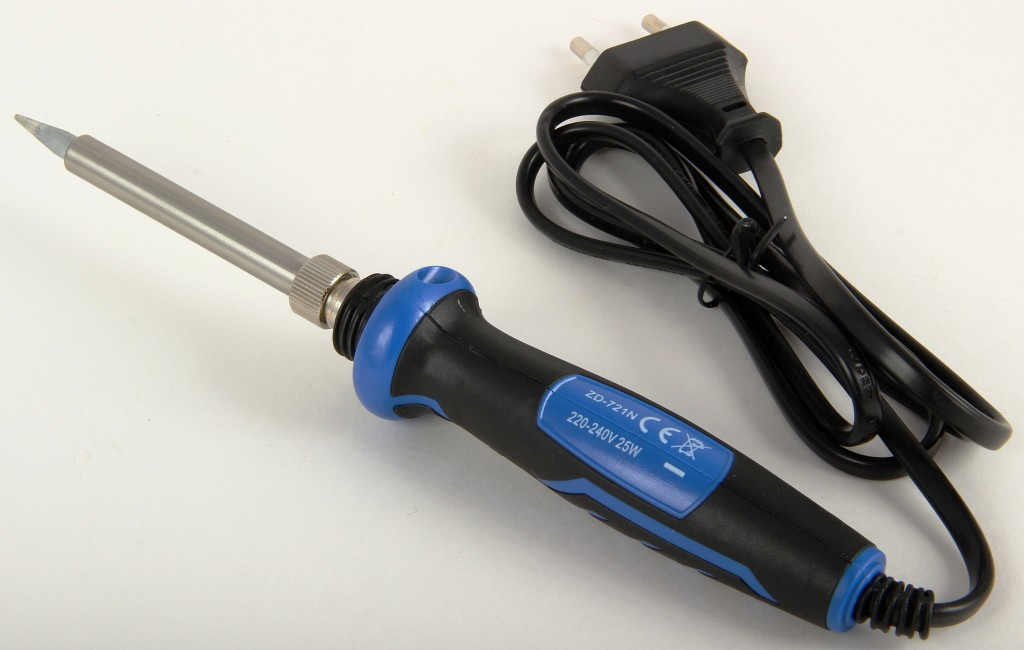
\includegraphics[width=\columnwidth]{00/fig/ZD-721N.jpg}}
\textbf{Паяльник 220В 25Вт ZD-721N 175\,р.}

\columnbreak

\noindent\href{http://voltmaster-samara.ru/catalog/product/00047380/}{
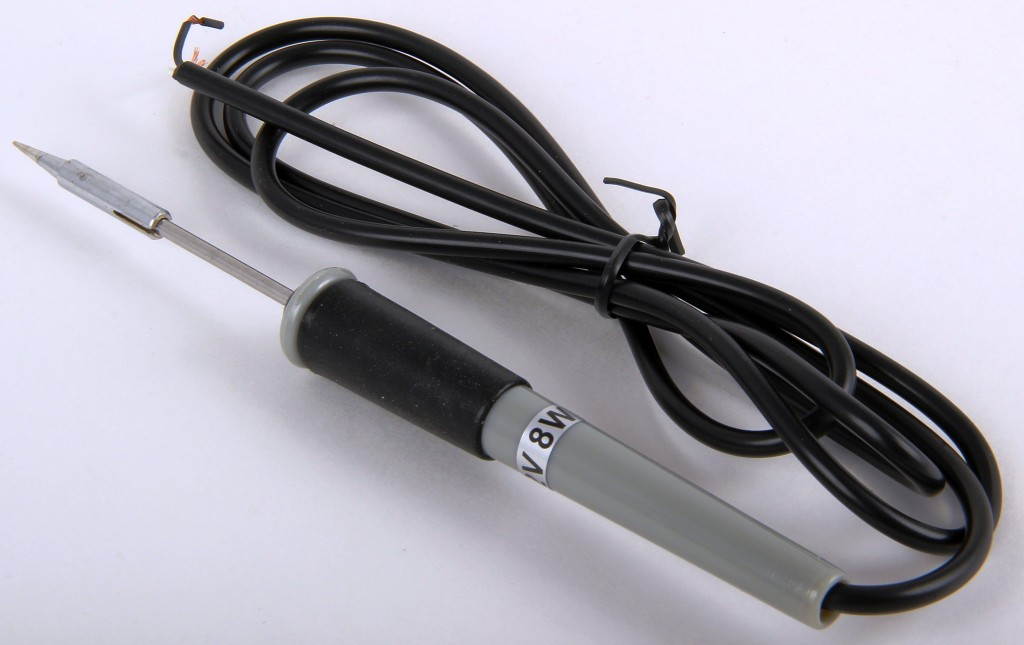
\includegraphics[width=\columnwidth]{00/fig/Iron8W.jpg}}
\textbf{Паяльник для станции ZD-927 12\,В 8\,Вт 85\,р.}
\end{multicols}

\subsubarticle{Паяльная станция}

\begin{multicols}{2}
Если не жалко 500\,р, берите ZD-927 целиком, внутри простейший регулятор
мощности, и вам не понадобится источник питания на 12\,В, который вы еще не
сделали. \emph{Но труъ путь\ --- конечно собрать свой паяльник целиком, из
нихрома, жала из толстой проволоки или медной шины, и самостоятельно выточенной
ручки.}

\columnbreak

\noindent\href{http://voltmaster-samara.ru/catalog/product/00073790/}{
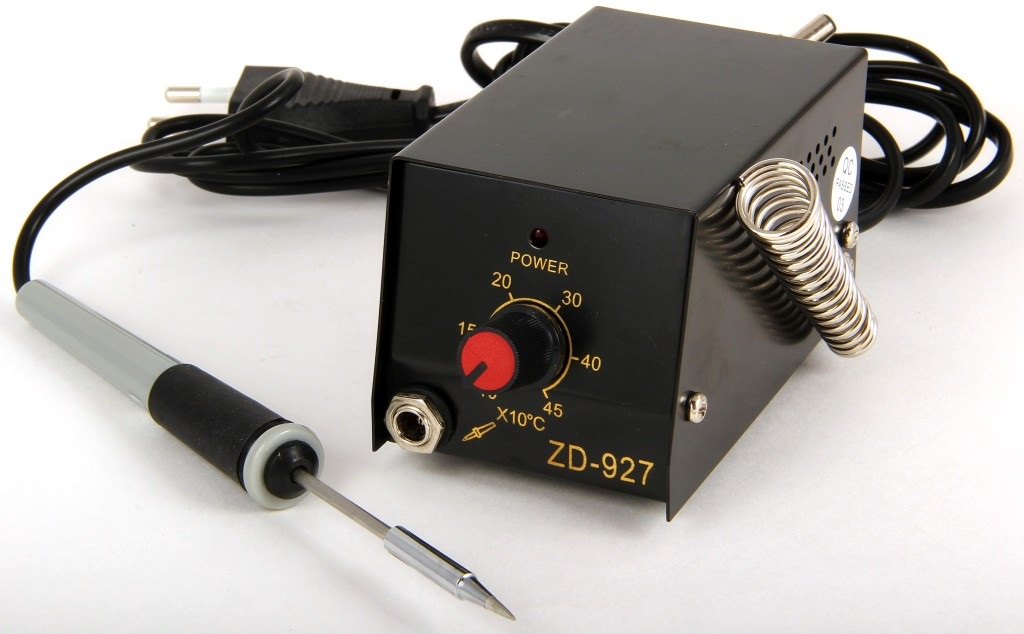
\includegraphics[width=\columnwidth]{00/fig/ZD927.jpg}}
\textbf{Паяльная станция ZD-927 520\,р.}
\end{multicols}

Паяльные станции типа Lukey 702/853D (3000+\,р) естественно не рассматриваем
\smiley. Для работы или регулярного хобби паяльная станция с феном, а может даже
и встроенным источником питания, вещь незаменимая, и не такая уж дорогая, но для
\scr а слишком технологичная.

\begin{multicols}{2}
\noindent\href{http://voltmaster-samara.ru/catalog/product/00073444/}{
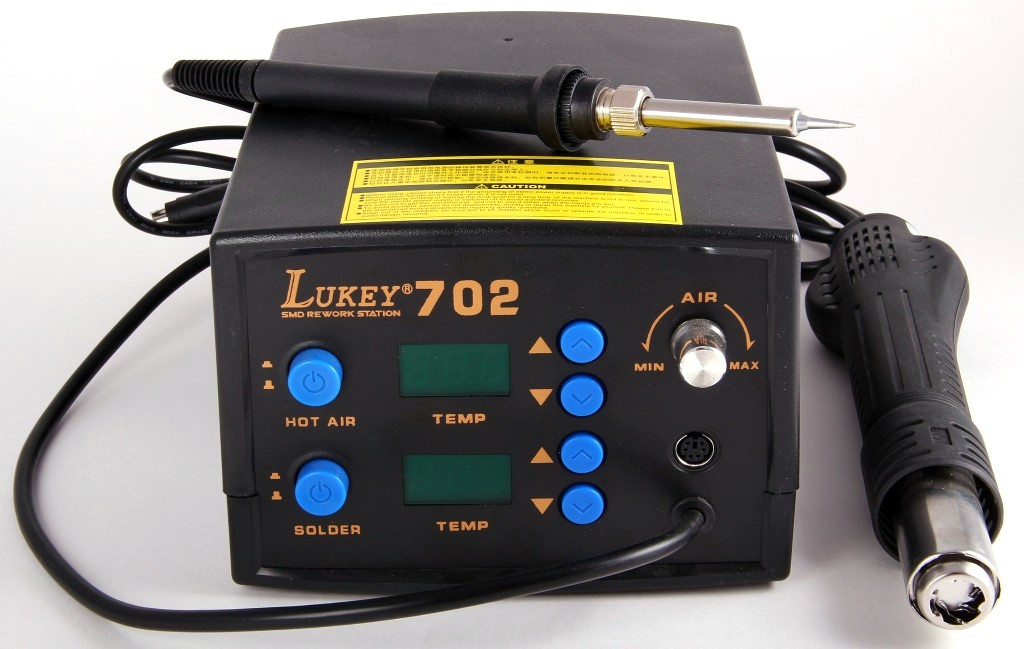
\includegraphics[width=\columnwidth]{00/fig/Lukey702.jpg}}
\textbf{Паяльная станция LUKEY 702 3100\,р.}

\columnbreak

\noindent\href{http://shop.siriust.ru/product\_info.php/cPath/23\_28\_269/products\_id/15290}{
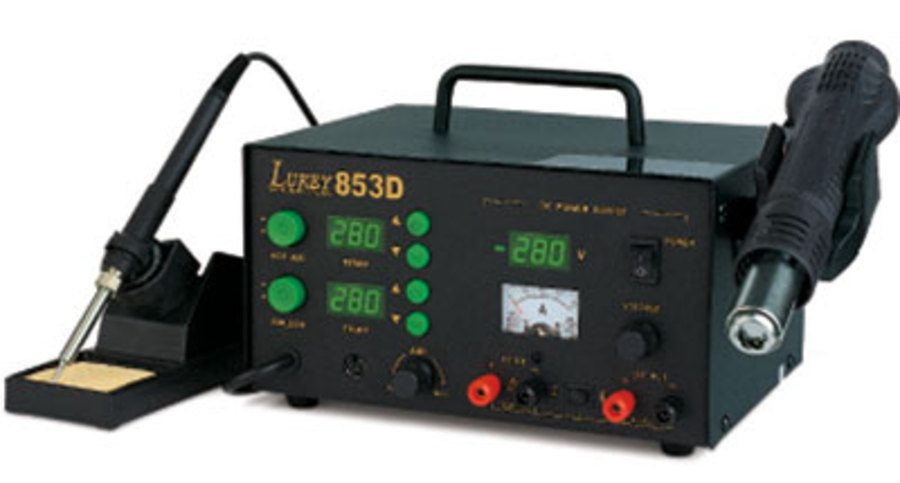
\includegraphics[width=\columnwidth]{00/fig/Lukey853D.jpg}}
\textbf{Паяльная станция LUKEY 853D с источником питания 5200\,р.}

\end{multicols}

\subarticle{Жвигатель}

\begin{multicols}{2}
\noindent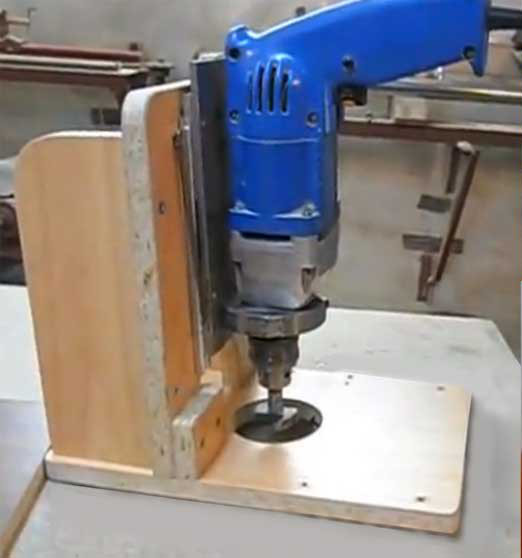
\includegraphics[width=\columnwidth]{00/fig/DrelBoren.jpg}

\noindent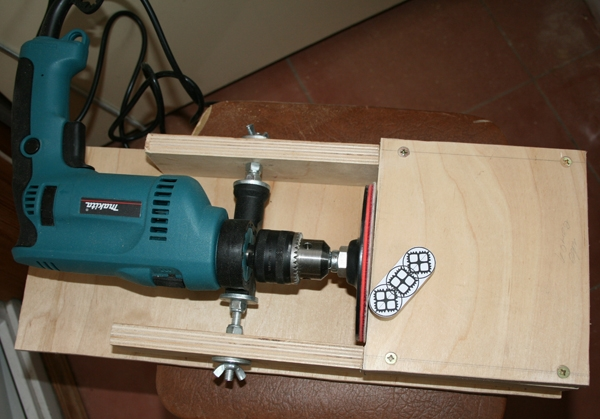
\includegraphics[width=\columnwidth]{00/fig/DrelShliph.jpg}

\noindent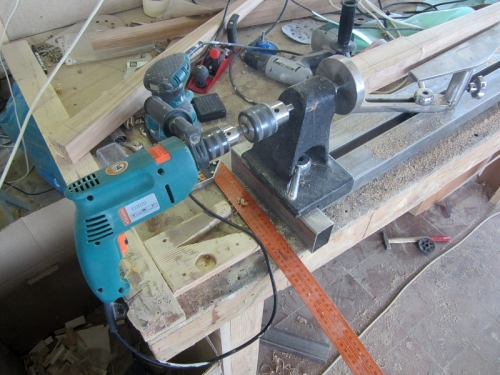
\includegraphics[width=\columnwidth]{00/fig/DrelLathe.jpg}

\noindent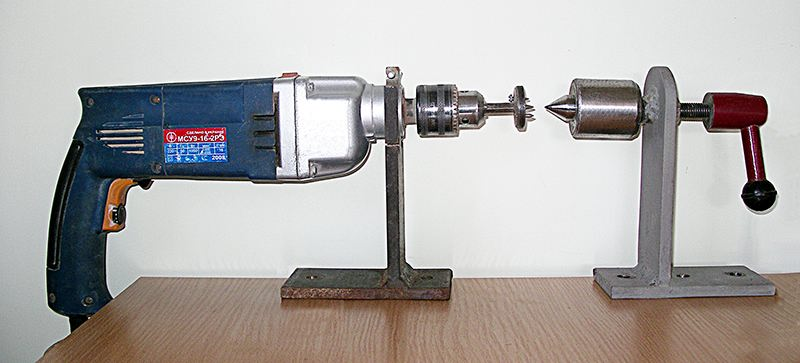
\includegraphics[width=\columnwidth]{00/fig/DrelLathe2.jpg}
\end{multicols}

Первый кандидат на место универсального электропривода достается той
самой дрели, не забываем об обязательном наличии 43\,мм монтажной шейки.
Достоинство дрели как привода\ --- прямое подключение к сети, встроенный
редуктор, есть модели с простой регулировкой оборотов, резьба и отверстие под
винт на валу, в комплекте есть патрон для зажима мелких деталей в
точилке\footnote{\ БЗП удобен, патрон с ключем дает лучший зажим и возможно
точнее}

Ограниченно доставаемые двигатели от стиральных машин, отличаются мощностю и
оборотистостью, особенно от старых моделей. Часто доступны сразу с готовым
шкивом на валу, который иногда проще использовать, чем снять.

\bigskip
Автозапчасти: привод печки Камаза, двигатель постоянного тока 24\,В
  50\,Вт

\begin{multicols}{2}
\noindent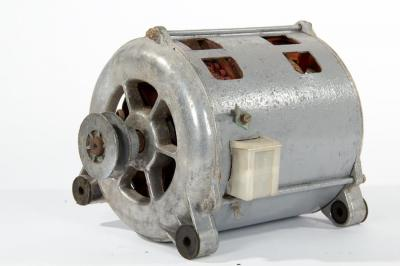
\includegraphics[width=\columnwidth]{00/fig/VyatkaDvig.jpg}
\textbf{Жвигатель Вятка-Автомат 19??\,г.}

\noindent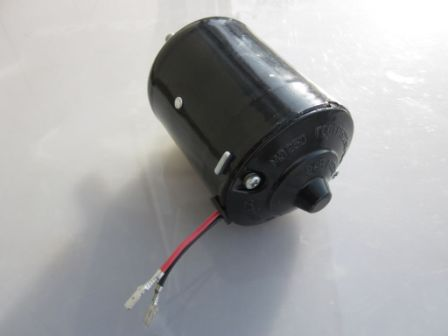
\includegraphics[width=\columnwidth]{00/fig/KamazDvig.jpg}
\textbf{Двигатель печки Камаза}

\noindent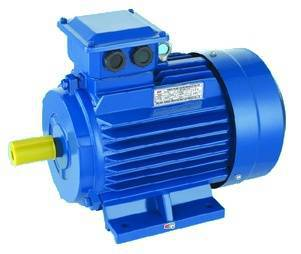
\includegraphics[width=\columnwidth]{00/fig/AIRE.jpg}
\textbf{АИРЕ 56 B2, 0.2\,КВт}

\end{multicols}

\bigskip
Новые асинхронные двигатели АИРЕ 56 B2/B4 (3000/1500 об.)
с заводским конденсатором, подключается к сети $\sim$220\,В, цена от 2500\,р.
С ростом размеров и мощности цена резко повышается.
Следует обратить внимание на возможность монтажа на дополнительный фланцевый
подшипниковый щит, (?) с моделями АИРЕ 80.

\subsubarticle{Фрезерный шпиндель}

Съемные фрезерные шпиндели, поставляются отдельно или в комплекте с
насадкой ручного фрезера по дереву. Лучшие, со стальной шейкой\ --- Kress,
активно применяются хобби-ЧПУшниками.

\begin{multicols}{2}

\noindent\href{http://kress-shop.ru/product/frezernyj-dvigatel-530-fm-kress-06082302/}{
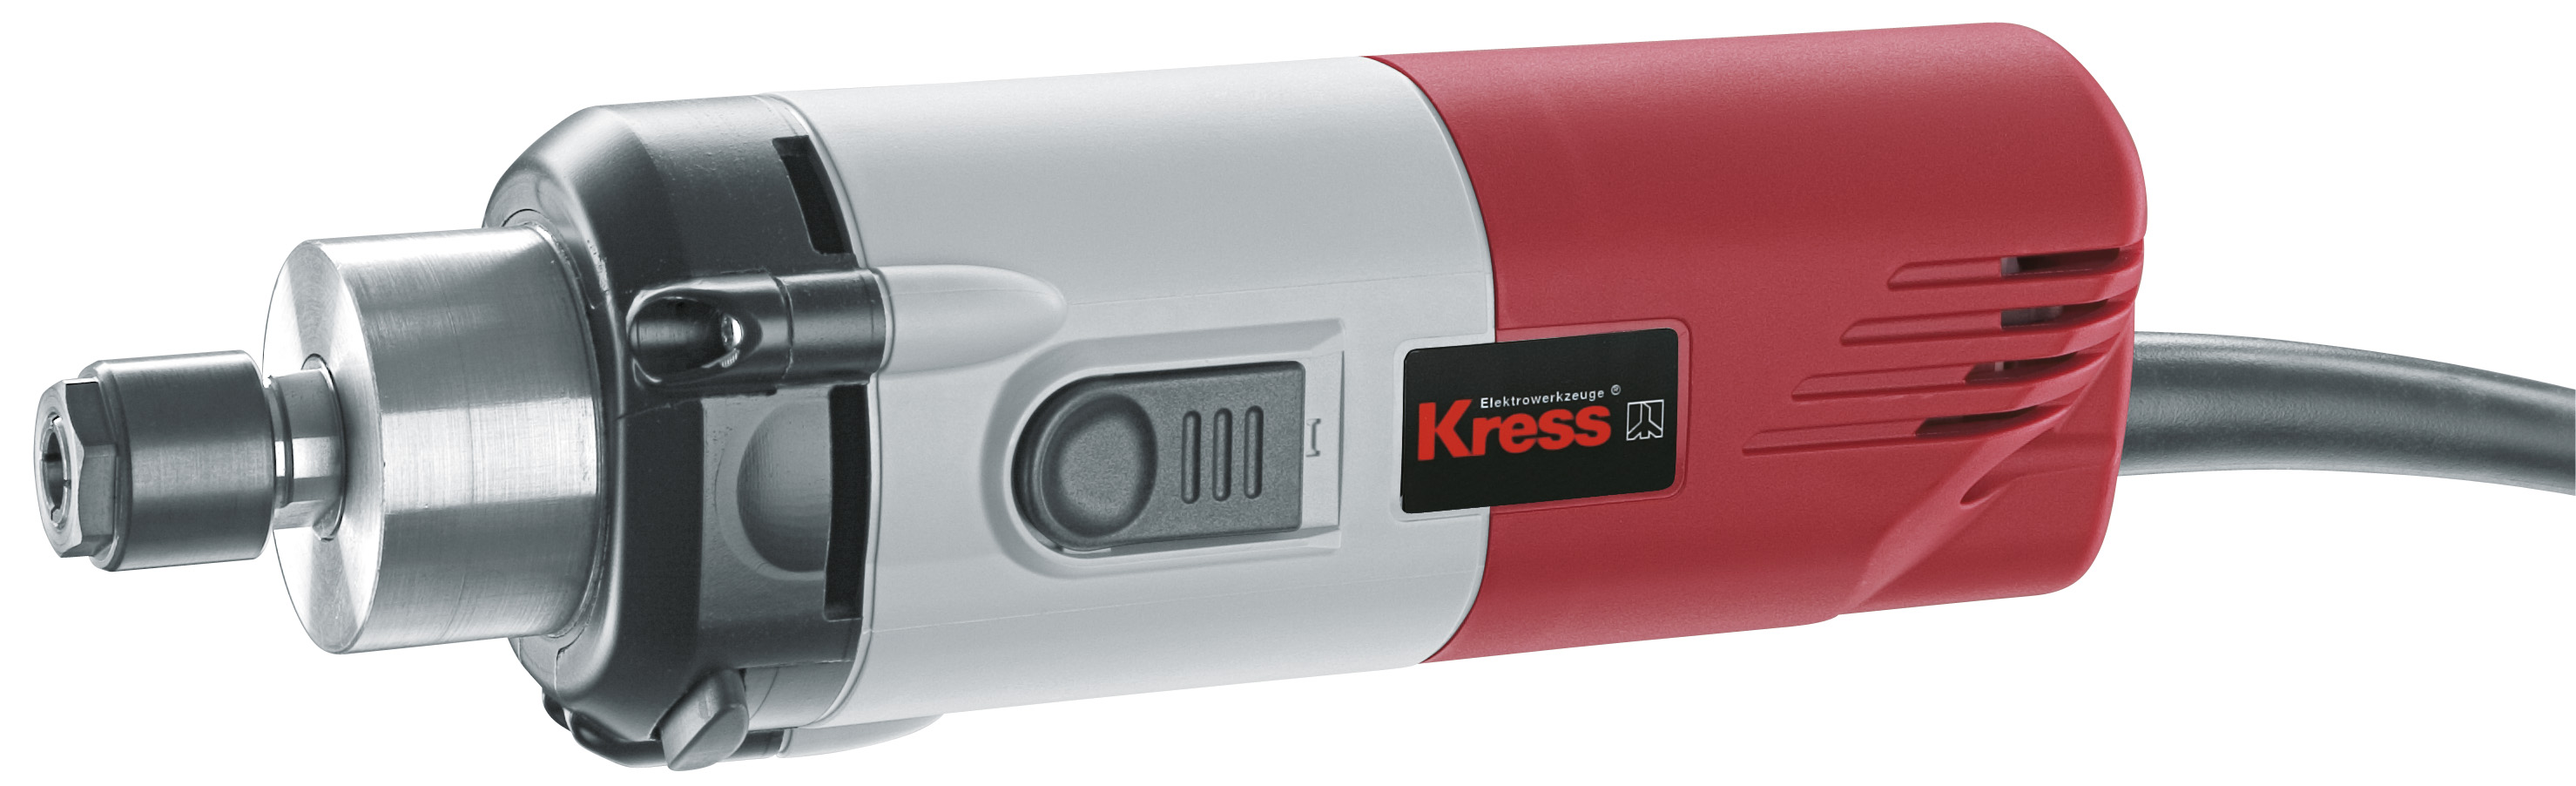
\includegraphics[width=\columnwidth]{00/fig/Kress530.jpg}}
\textbf{Фрезерный двигатель KRESS 530/800/1050 FM(E) 5600+\,р.}

\noindent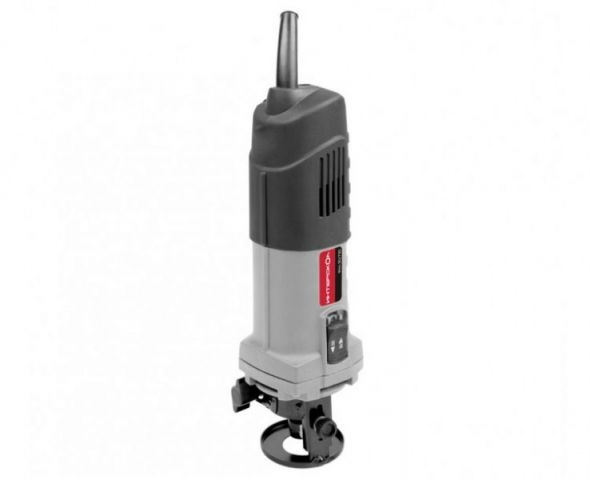
\includegraphics[width=\columnwidth]{00/fig/Interskol30.jpg}
\textbf{Шпиндель Интерскол ФМ-30/750 /снят с производства/}

\end{multicols}

Попроще и сильно дешевле делал Интерскол, иногда попадается noname.

Недостаток как универсального привода\ --- они высокоскоростные,
возникают проблемы с понижающими передачами. Применение\ --- приводной
высокоскоростной инструмент: боры, фрезы по дереву, микроинструмент для
граверов (микродиски, шарошки).

\begin{multicols}{2}
\noindent\href{http://www.kuvalda.ru/catalog/1867/27920/}{
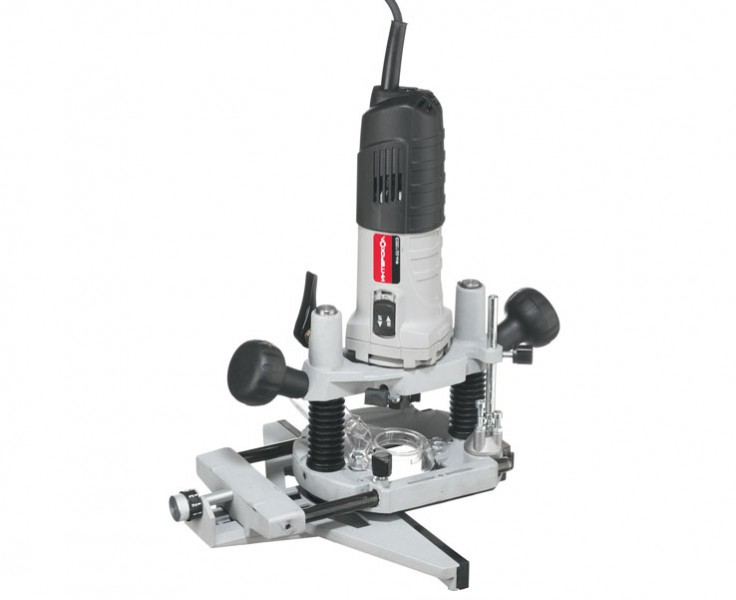
\includegraphics[width=0.5\columnwidth]{00/fig/InterskolFM55.jpg}}
\textbf{Фрезер сетевой Интерскол ФМ-55/1000 Э 5050\,р.}

\columnclear

\noindent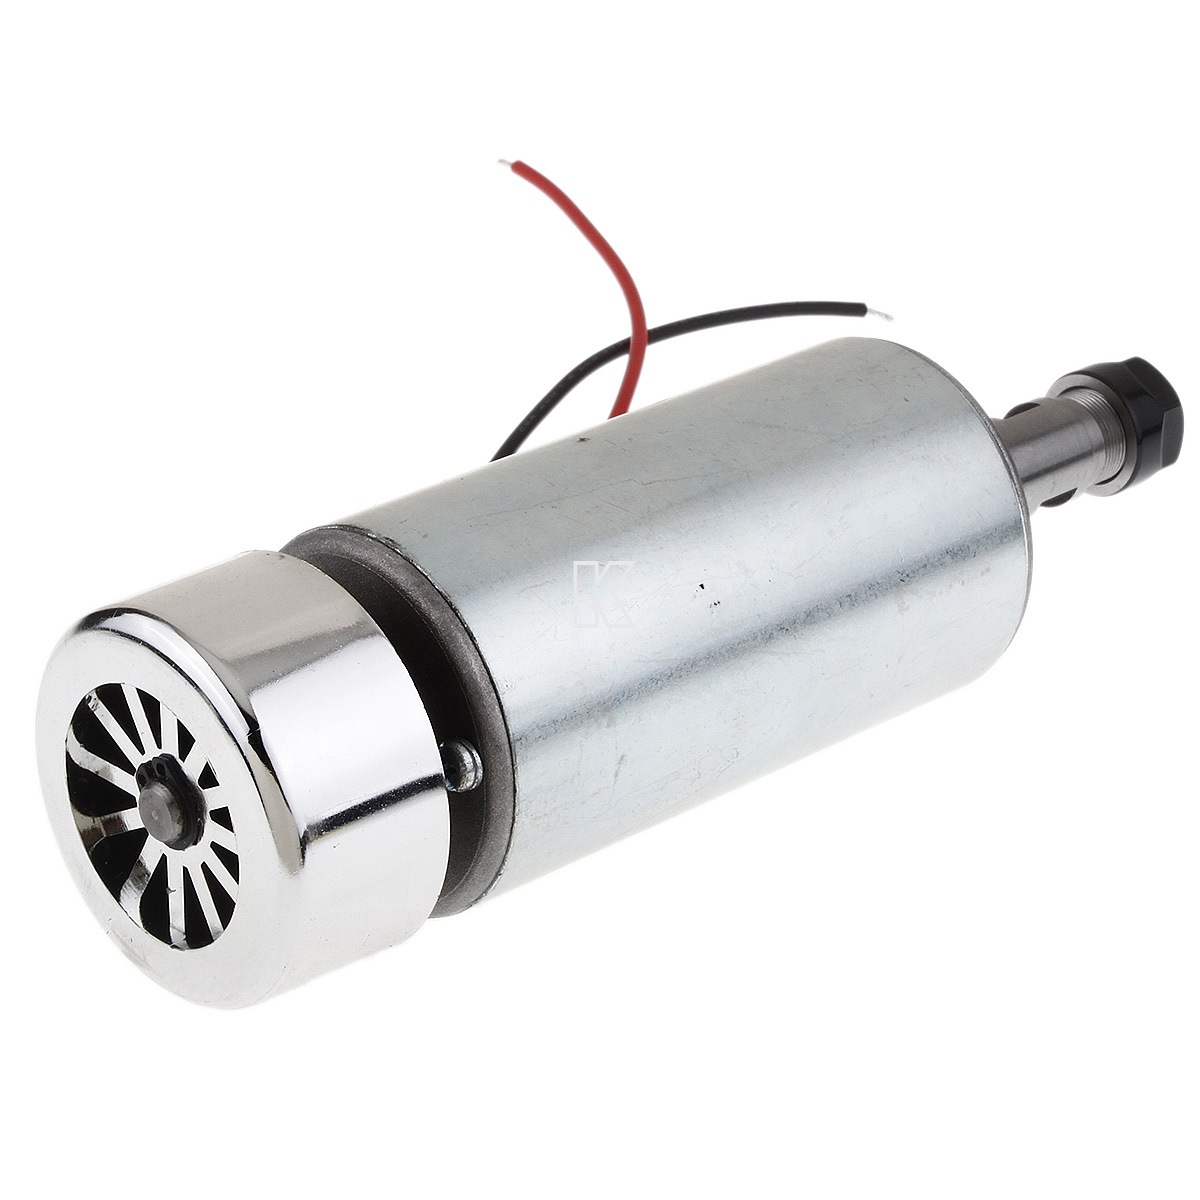
\includegraphics[width=0.5\columnwidth]{00/fig/ER11.jpg}
\end{multicols}

Китайские воздушные шпиндели постоянного тока с цанговыми патронами ER11:
привод для сверлилки и микроинструмента. Требуют источник питания
постоянного тока 9$\div$48\,В.

\subarticle{Ручной инструмент}

По мелкому ручному инструменту вопрос открыт.

Учитывая доступность и наличие дешевых вариантов, стоит ли использовать старый
опыт мастеров-ремесленников, когда ученику давали только напильник, и он сам
должен был изготовить себе весь инструмент\,?

По крайней мере, вот этот вариант точно не подходит \smiley:

\noindent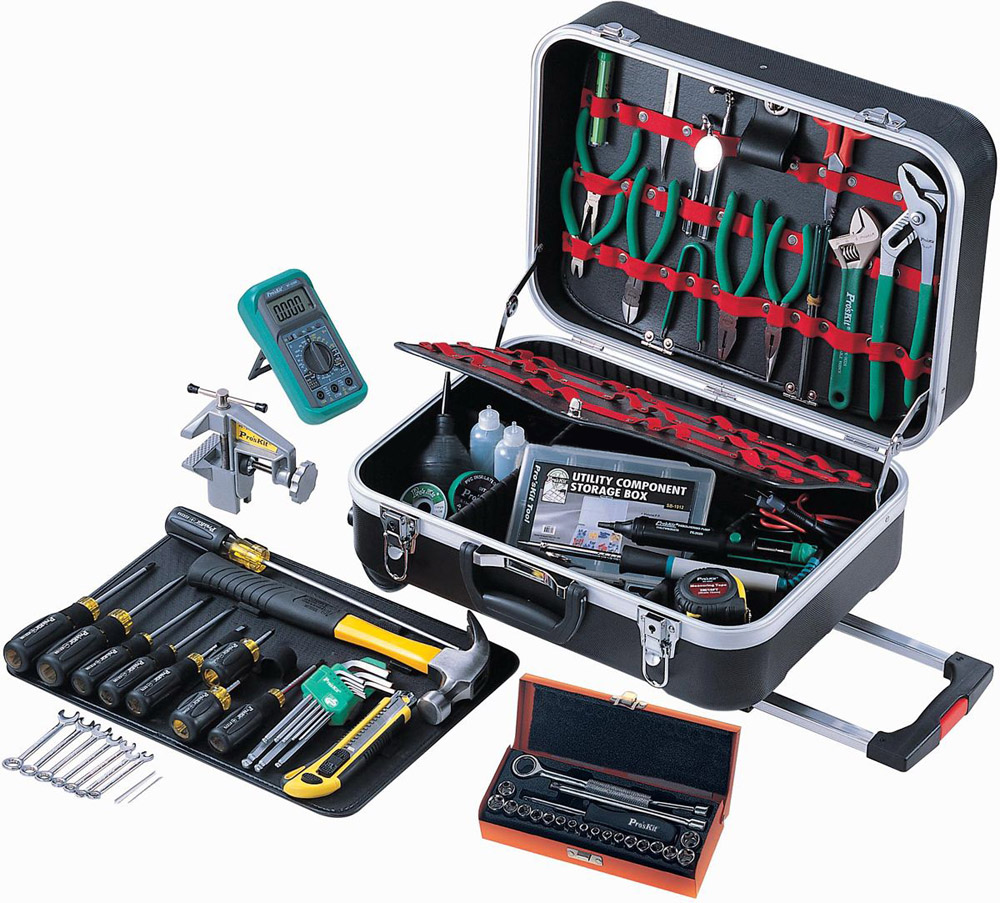
\includegraphics[width=\columnwidth]{00/fig/PK5308BM.jpg}
\textbf{PK-5308BM универсальный набор инструментов Pro'sKit}

Но пара надфилей, заточной камень на дрель, комплект сверел и несколько листов
наждачки вполне допускаются \smiley.

Если хочется посложнее, можно ограничиться только парой электродвигателей:
\begin{enumerate}
  \item
относительно медленный высокомоментный АИРЕ 56 B2/4 на силовой привод и
\item
высокоскоростной 10+ тыс.об$^{-1}$ для сверления, шлифования насадками и т.п.
операции допускающие работу с большими скоростями

\end{enumerate}

\subarticle{Pro'sKit}

Отдельного обзора заслуживает инструмент и наборы
\href{http://www.proskit.com/}{Pro'sKit}
 / \href{http://www.proskit.msk.ru/index.html}{ru}:

\subsubarticle{Инструмент до 1000\,В}

Для электромонтажных работ обязательно приобретите комплект
высоковольтного инструмента до 1000\,В:

\begin{multicols}{2}
\noindent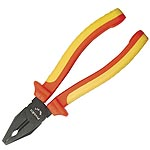
\includegraphics[width=\columnwidth]{00/fig/pros/PM-911.jpg}
\textbf{PM-911 Пассатижи 1\,кВ}

\noindent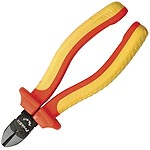
\includegraphics[width=\columnwidth]{00/fig/pros/PM-917.jpg}
\textbf{PM-917 Кусачки (бокорезы) 1\,кВ}
\end{multicols}

\subsubarticle{Хранение}

\begin{multicols}{2}

\noindent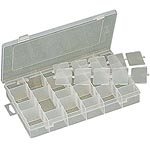
\includegraphics[width=\columnwidth]{00/fig/pros/103-132D.jpg}
\textbf{103-132D Кассетница для деталей и компонентов}

\noindent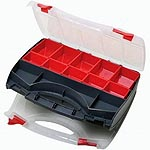
\includegraphics[width=\columnwidth]{00/fig/pros/SB-3428SB.jpg}
\textbf{SB-3428SB Портативная кассетница для саморезов и т.п.}
\end{multicols}

\subsubarticle{Радиомонтаж}

\begin{multicols}{2}

\noindent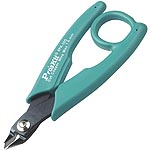
\includegraphics[width=\columnwidth]{00/fig/pros/8PK-30D.jpg}
\textbf{8PK-30D Кусачки миниатюрные}

\noindent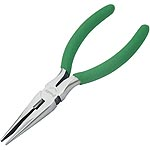
\includegraphics[width=\columnwidth]{00/fig/pros/1PK-709.jpg}
\textbf{1PK-709 Длинногубцы-кусачки}

\noindent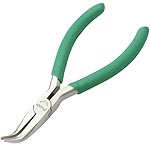
\includegraphics[width=\columnwidth]{00/fig/pros/1PK-055S.jpg}
\textbf{1PK-055S Длинногубцы изогнутые}

\noindent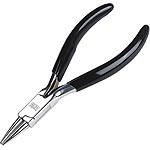
\includegraphics[width=\columnwidth]{00/fig/pros/1PK-29.jpg}
\textbf{1PK-29 Круглогубцы}

\noindent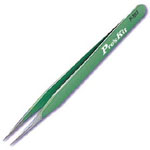
\includegraphics[width=\columnwidth]{00/fig/pros/1PK-101T.jpg}
\textbf{1PK-101T Пинцет прямой}

\noindent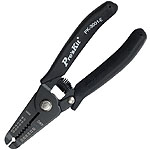
\includegraphics[width=\columnwidth]{00/fig/pros/1PK-3001E.jpg}
\textbf{1PK-3001E Клещи для зачистки проводов прецизионные (стриппер)}

\noindent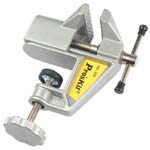
\includegraphics[width=\columnwidth]{00/fig/pros/PD-374.jpg}
\textbf{PD-374 Тиски на струбцине}

\end{multicols}


\subsubarticle{Наборы}

\begin{multicols}{2}
\noindent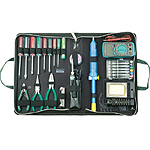
\includegraphics[width=\columnwidth]{00/fig/pros/1PK-616B.jpg}
\textbf{1PK-616B Набор инструментов для электроники профессиональный}

\columnbreak

\noindent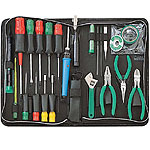
\includegraphics[width=\columnwidth]{00/fig/pros/1PK-813B.jpg}
\textbf{1PK-813B Набор базовых инструментов для электроники}
\end{multicols}

По личному опыту: в 1PK-813B не хватает мелкого мультиметра, стриппера
1PK-3001E, микрокусачек типа 8PK-30D, канифоли, ножа, настроечную отвертку
заменить индикаторной.

\subarticle{Прочие}

Попалась интересная недорогая отвертка:

\begin{multicols}{2}
\noindent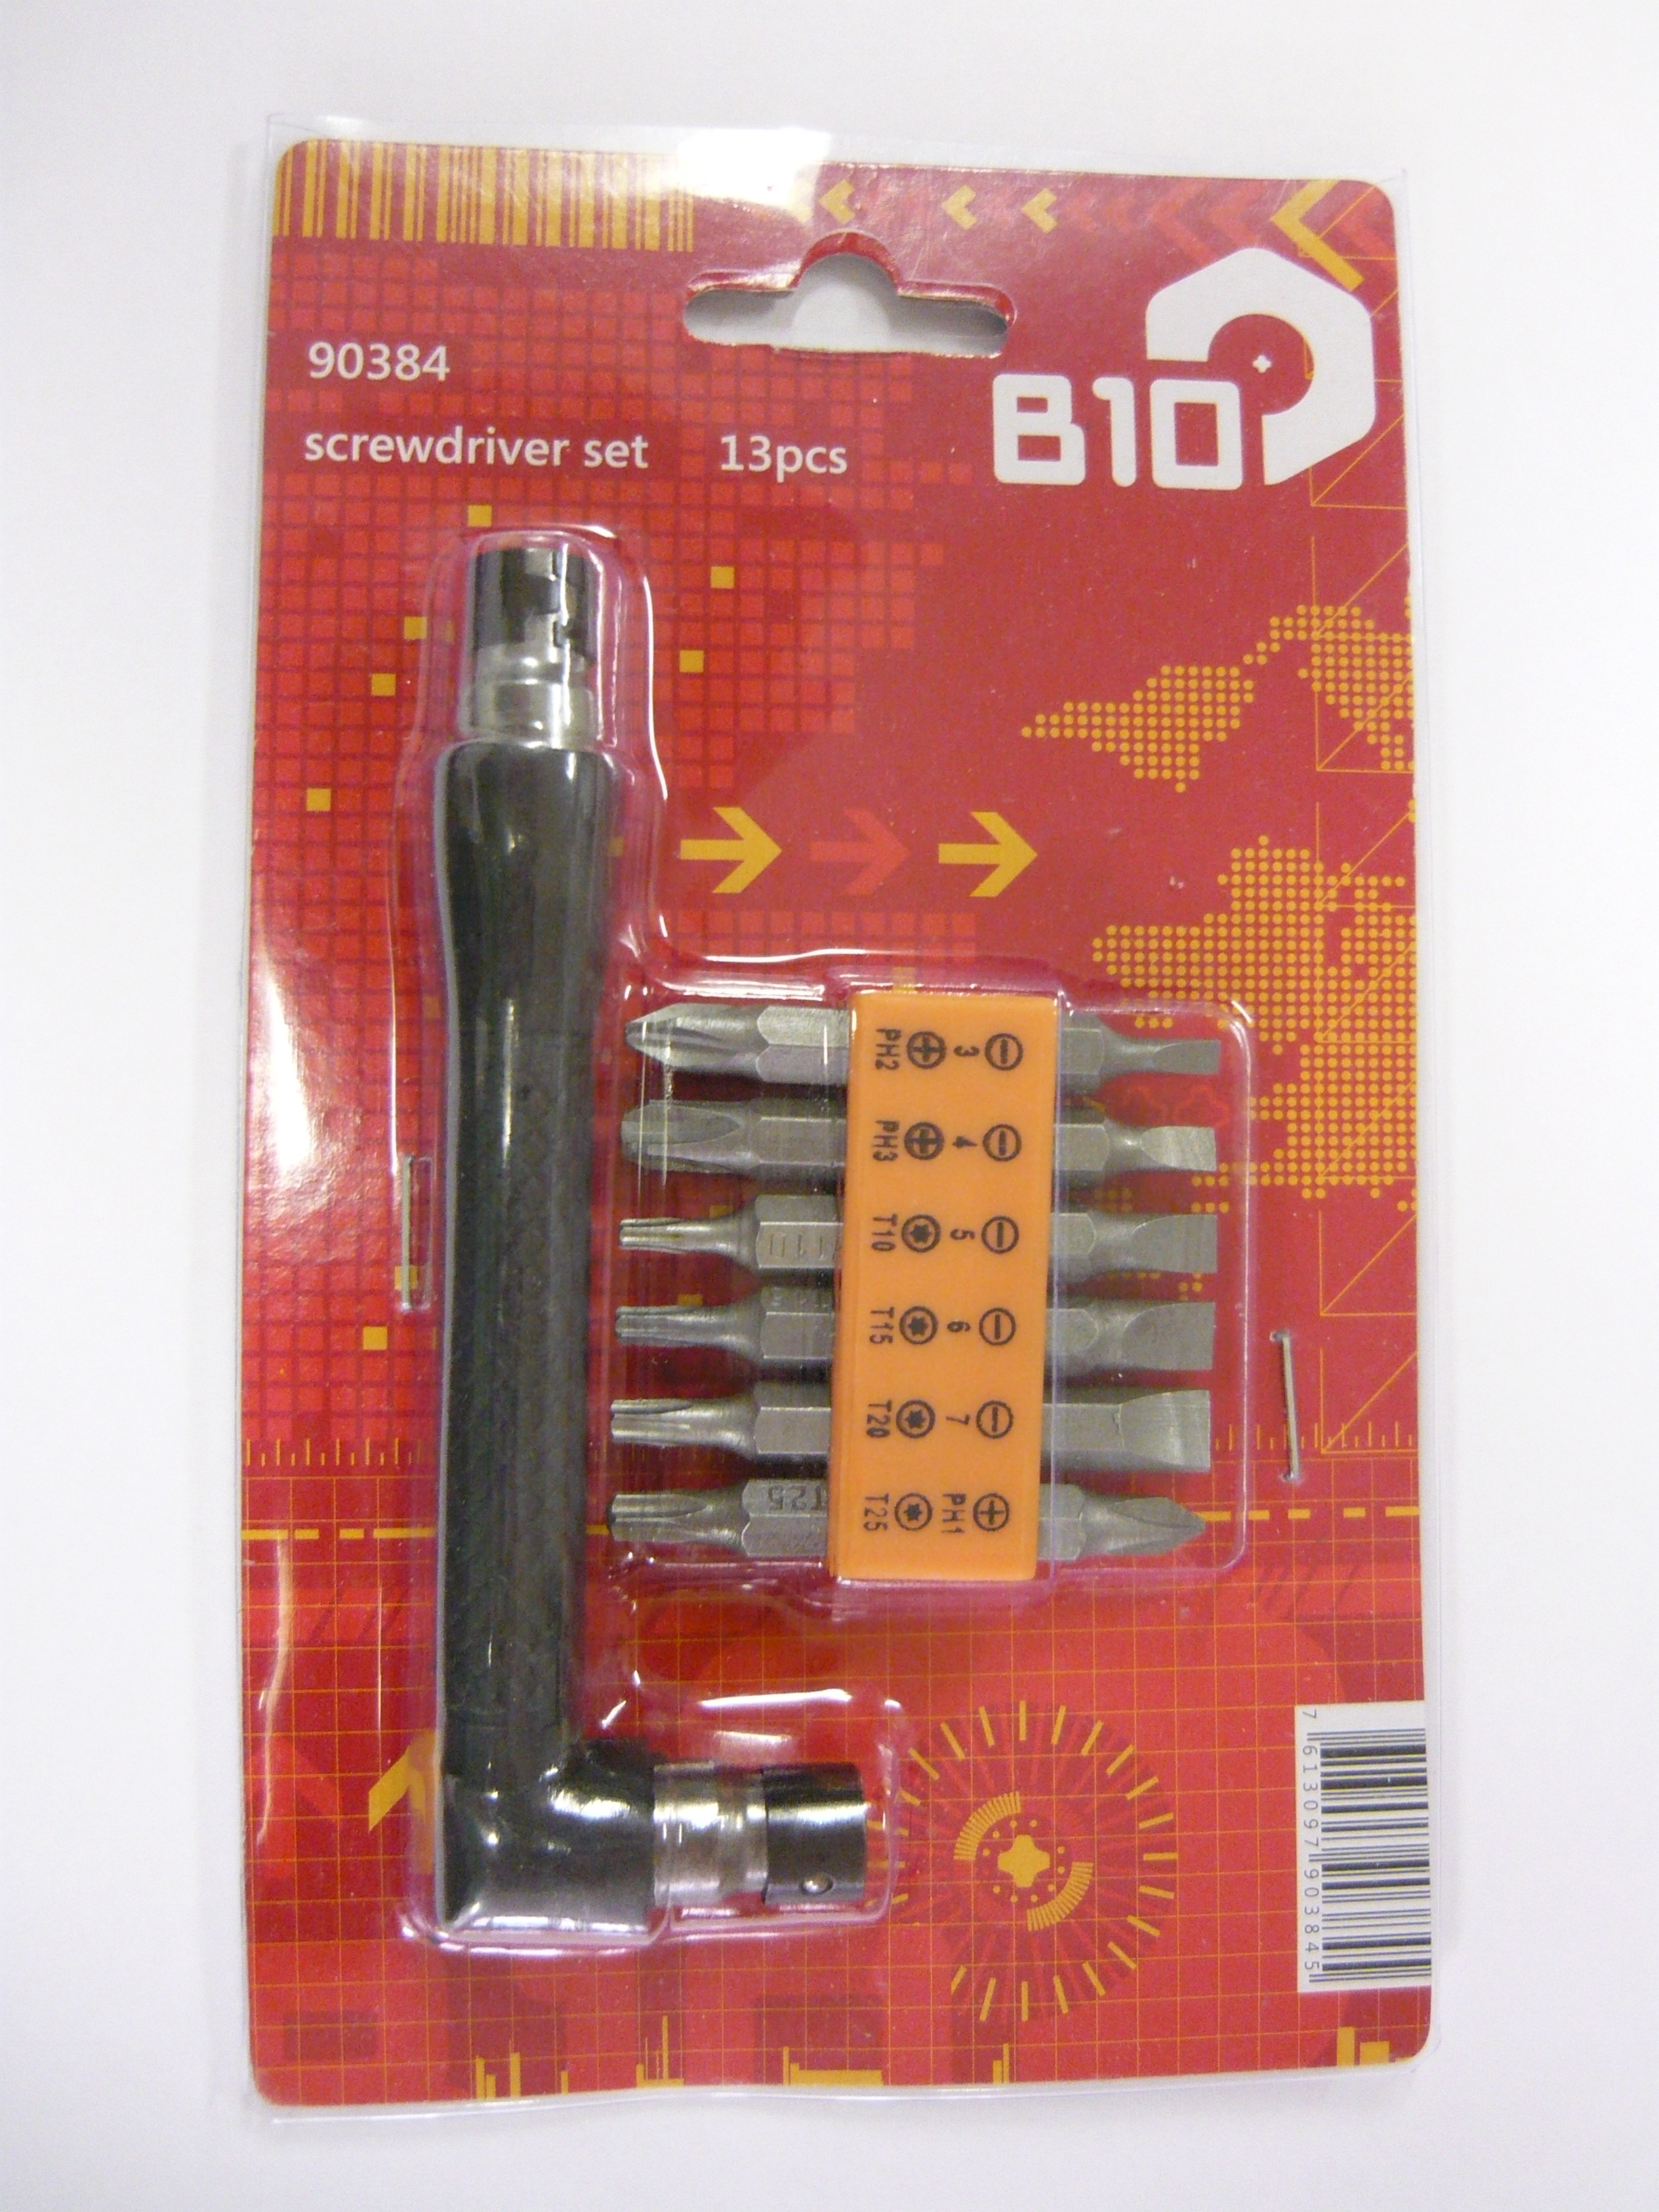
\includegraphics[width=0.9\columnwidth]{00/fig/P1020966.jpg}

\noindent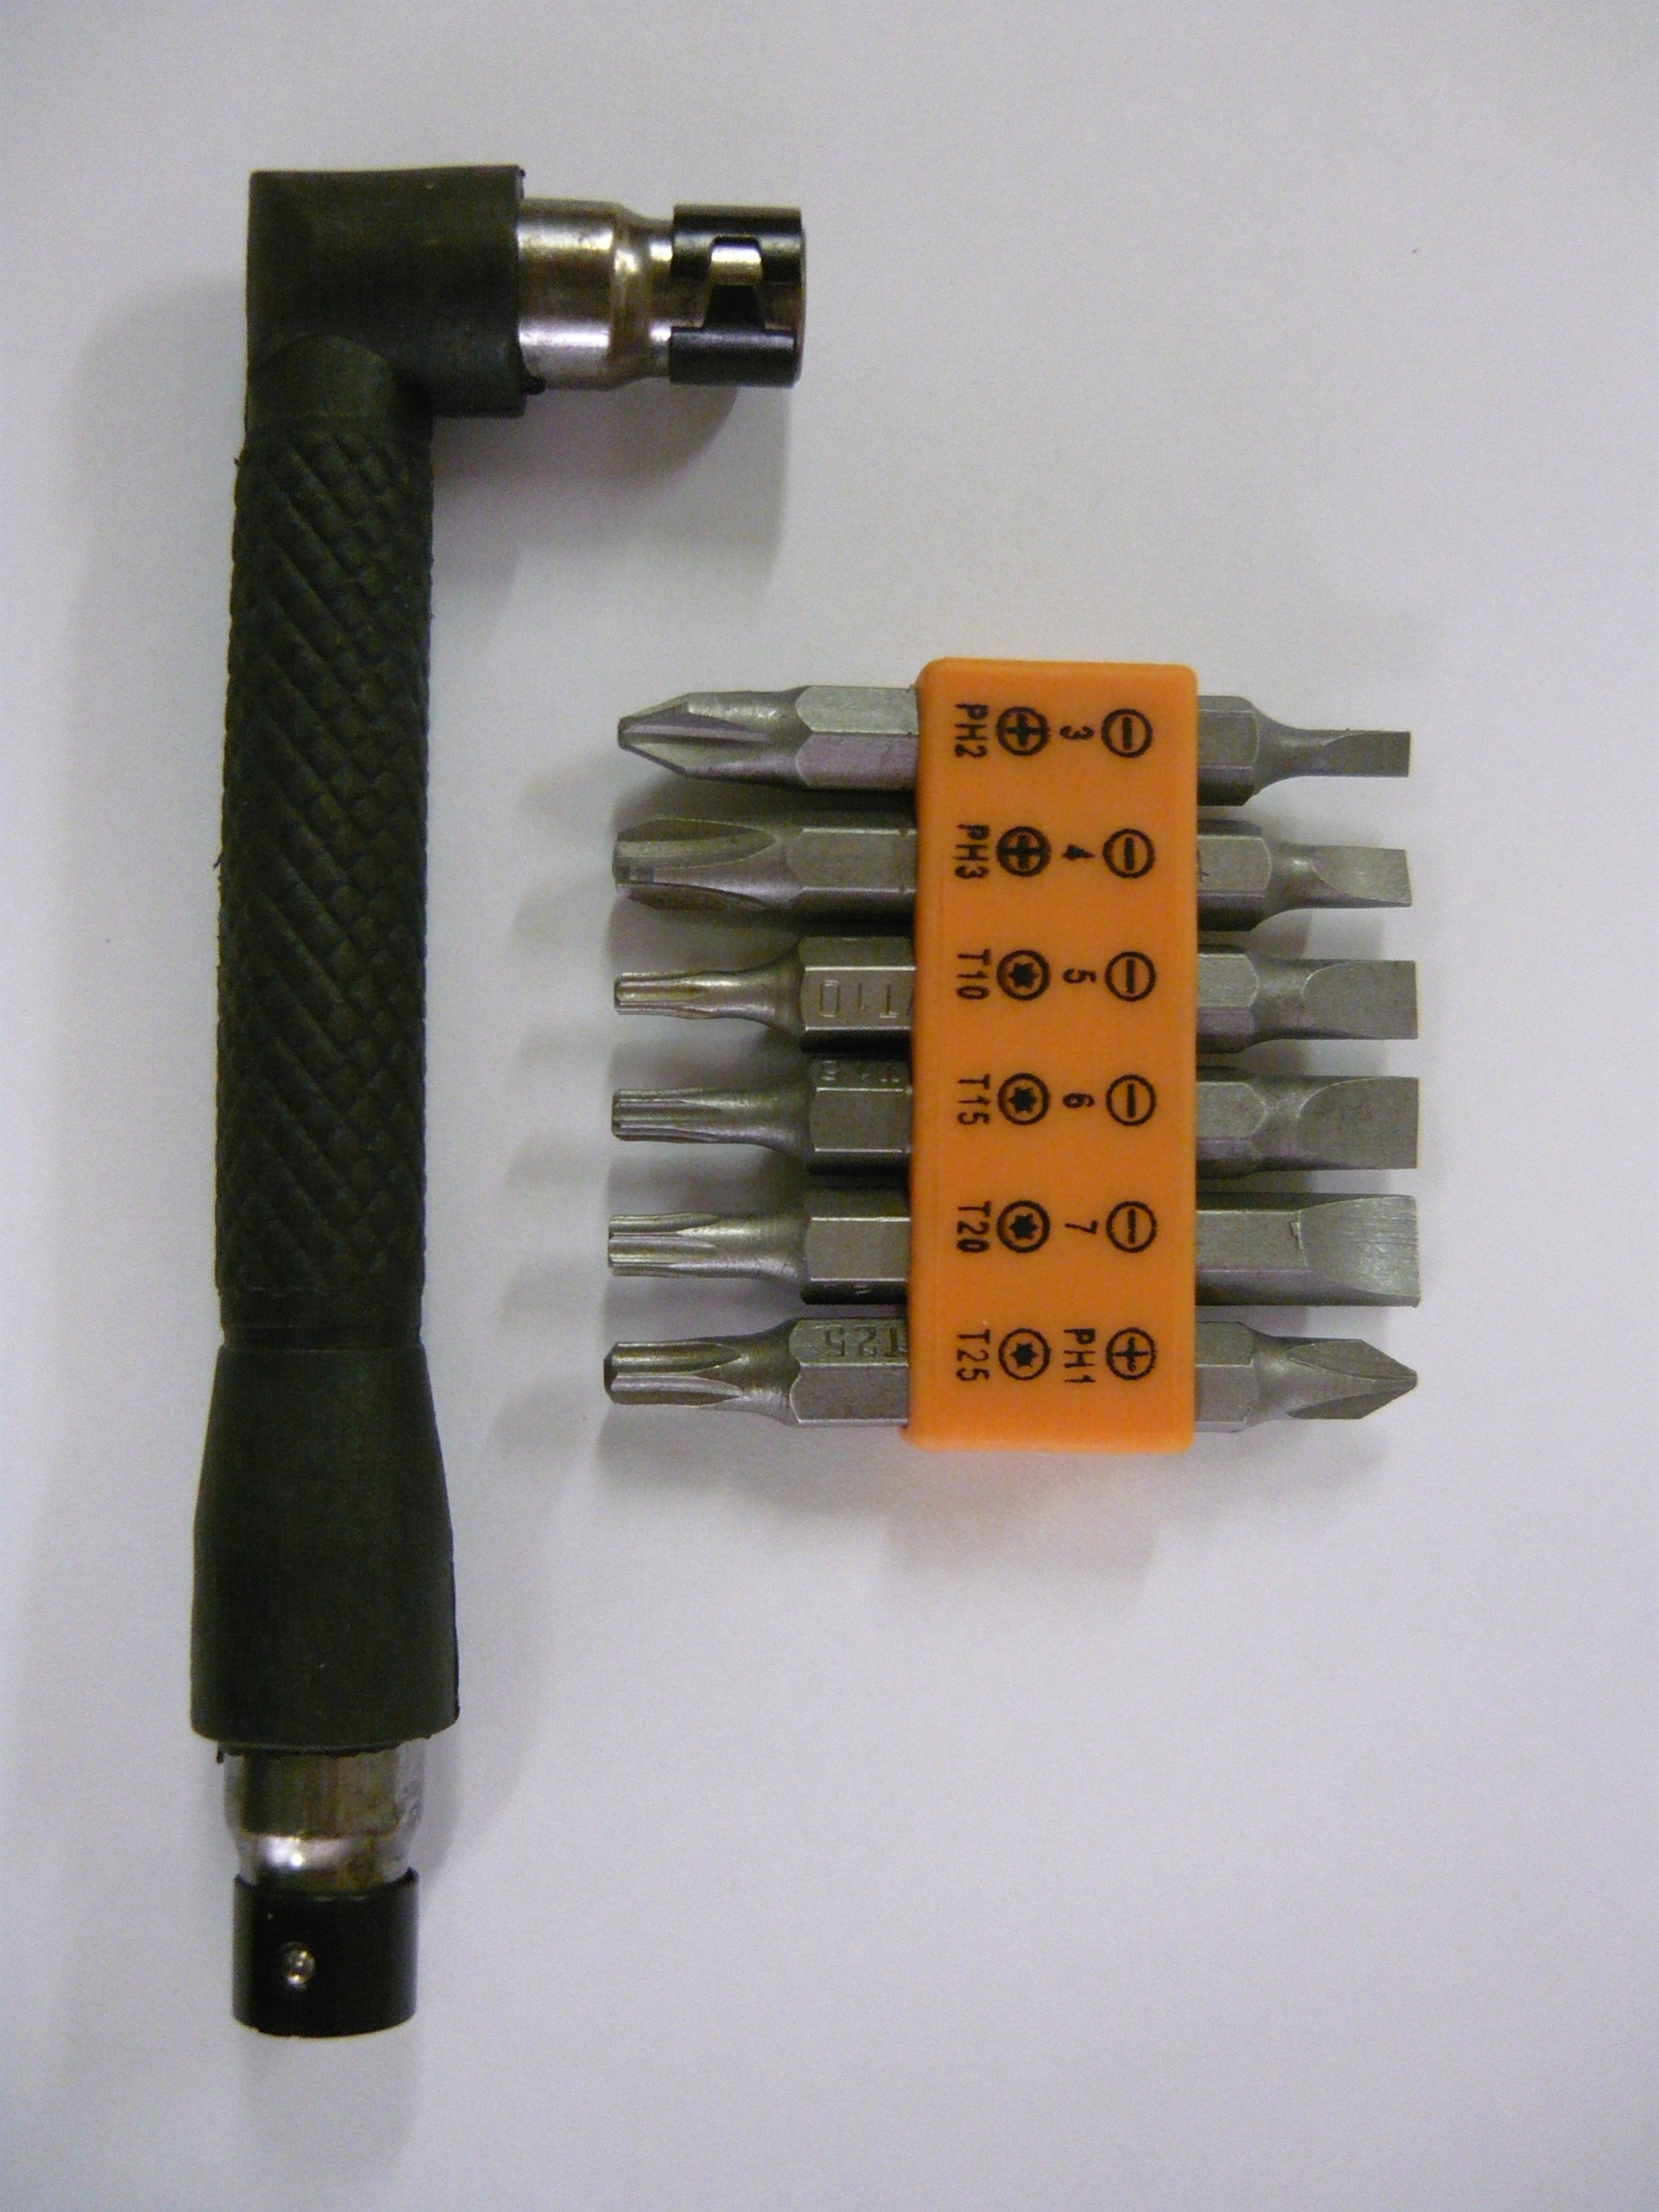
\includegraphics[width=0.9\columnwidth]{00/fig/P1020967.jpg}
\end{multicols}

Фиксация четкая, исполнение очень неплохое, позволяет добраться до узких мест.
Из минусов: ручка похоже не цельнометаллическая, при изломе есть риск 
распороть руку.

}{}
